%% USPSC-Introducao.tex

% ----------------------------------------------------------
% Introdução (exemplo de capítulo sem numeração, mas presente no Sumário)
% ----------------------------------------------------------
\chapter[Introduction]{Introduction}
\label{Introduction}

At the end of the 20th century, there was a fundamental transformation in the methods used to perform surgical procedures. For many interventions, the invasive nature has been considerably reduced, bringing superior results such as a better survival rate, lower incidence of complications, and faster recovery in terms of functional health and quality of life. This emphasis on less invasive approaches, also known as minimally invasive surgery (MIS), has been gaining momentum and has been the subject of intensive research and development of new surgical techniques in recent years \cite{minimal}.

In 1985 there was the first interaction between medicine and robotics with the \textit{PUMA\texttrademark} manipulator focused on brain biopsies. Surgical interventions expanded their horizons with the \textit{ da Vinci\texttrademark} robot, enabling tasks to be carried out with precision and strength beyond human capacity and allowing surgeons to perform tasks impossible to perform without robots \cite{morrell2021history}.

% @gui maybe one for Zeus?

The Da Vinci® Surgical System has had a positive impact on surgery. Other examples include the Renaissance® System. The MAKO has been shown to increase the accuracy rate, and provides precision and eliminates the need for hand instruments in orthopedic procedures. Showing that robotic systems have contributed to significant improvements in the results of surgical operations, reducing trauma for patients, and accelerating postoperative recovery \cite{Meng2014}.

This work focuses on the development of a robotic system for the treatment of epilepsy through SEEG surgery. Robots such as ROSA, Neuromate and Circ are capable of carrying out such treatment. However, each of them has its disadvantage. To better understand the context of this development, it is necessary to understand the characteristics of epilepsy (Section \ref{sec:epi}), the types of crises and their impact on the patient's life, as well as the existing treatment methods (Section \ref{sec:methods}).

\section{Epilepsy}\label{sec:epi}

% @gui one for what is epilepsy
%...
\textit{Epilepsy} is a chronic brain disease characterized by a long-lasting predisposition to generate seizures, not caused by any immediate insult to the central nervous system, and by the neurobiological, cognitive, psychological, and social consequences of recurrences of seizures \cite{beghi2020epidemiology}. This is the most common neurological disease worldwide, affecting different social classes, races, ages, and geographic locations \cite{ngugi2010estimation}.

% what is epilepsy seizures
The definition of \textit{epileptic seizures} is: repeated and transient episodes that manifest themselves through patterned behaviors, mirroring the underlying neural processes associated with the condition \cite{fisher2005epileptic}. Although all people with epilepsy experience seizures, not all individuals with seizures have epilepsy. Epileptic seizures can also occur after an acute injury to the central nervous system (CNS) of structural, systemic, toxic or metabolic origin. These events are considered acute manifestations of the insult and may not occur when the underlying cause has been removed or the acute phase has passed \cite{beghi2010recommendation}.

% types of epilepsy seizures
Epileptic seizures are categorized according to three main characteristics: origin in the brain, state of consciousness during the seizure and level of body movement. Seizures can be classified as focal or generalized based on the first characteristic. The second characteristic considers whether consciousness is intact or impaired during the seizure, while the third characteristic refers to body movement, which may present motor or non-motor reactions \cite{beghi2020epidemiology}.

Motor seizures encompass a variety of distinct manifestations. Atonic crises are characterized by a sudden and temporary loss of muscle tone, resulting in a sudden fall of the individual. On the other hand, tonic crises involve a sudden and prolonged increase in muscle tone, leading to intense stiffness. Clonic seizures are marked by rhythmic and repetitive muscle contractions, which can affect different parts of the body, while myoclonic seizures are characterized by rapid and sudden muscle contractions that can involve a specific muscle group or the entire body. Epileptic spasms, automatisms and hyperkinetic seizures are also categorized \cite{sarmast2020current}.

On the other hand, non-motor crises can present different forms of manifestation. They can be autonomic, involving dysfunctions in the autonomic nervous system, such as changes in blood pressure or heart rate. In addition, there may be crises of behavioral arrest, during which the individual may appear paralyzed or unable to perform voluntary movements. Cognitive crises affect cognitive function and may include memory lapses or mental confusion. Emotional crises are related to changes in the emotional state, such as feelings of fear, anxiety or euphoria. Finally, sensory crises affect the senses and can cause abnormal sensations, such as visual or auditory hallucinations \cite{sarmast2020current}.

\section{Treatment methods} \label{sec:methods}

% @gui one for what are the treatments
%...
Among patients with epilepsy, approximately 30\% experience drug-resistant seizures, representing a significant portion of the global population, estimated at 70 million people. In such cases, resective surgery appears as a viable therapeutic option. This procedure is considered in patients with disabling focal epilepsy who are unresponsive to drug treatment and whose seizures originate in a specific region of the brain that can be removed with minimal risk of neurological or cognitive dysfunction \cite{miller2013surgical}. Resective surgery offers the possibility of significantly improving the quality of life of these patients, providing adequate control of seizures and reducing dependence on high-cost and potentially harmful antiepileptic medications.

Correctly locating the focus of seizures is a crucial aspect in preparing for resective surgery in patients with epilepsy \cite{miller2013surgical}. Localization methods are applied to accurately determine the focal region, aiming to minimize the invasiveness of the surgery while seeking complete removal of the area of focus to cease seizures. Accuracy in locating the focus has a significant impact on the effectiveness of the surgical procedure, as it can help avoid undesirable consequences associated with the resection of unaffected areas. This is especially important, as the removal of critical areas of the brain can result in functional deficits, such as impairment of speech, memory, motor coordination, among other functions, depending on the location of the focus. Therefore, ensuring accurate location of the focus is essential to guarantee good surgical results and minimize potential adverse effects.


\subsection{Non-invasive video-EEG}

% @gui EEG
%...
Scalp EEG aims to investigate the cause of seizures in a non-invasive method. This procedure involves placing electrodes on the patient's scalp, using a cap or similar support, for monitoring in the interictal (between seizures), ictal (during seizures) and post-ictal (after seizures) periods. This configuration, with electrodes mounted superficially to the head, allows the measurement of the difference in electrical potential on the scalp caused by the electrical activity of neurons located mainly close to the skull. 32, 64 or 96 electrodes are placed across the entire surface of the scalp, each electrode corresponding to a channel. Systems with 256 channels are also adopted for more refined analyzes that require more channels per area \cite{Sun2023}. In summary, monitoring of seizure using scalp EEG as a preliminary analysis for diagnosis and location of the seizure is essential before proceeding to invasive methods \cite{miller2013surgical}.


\subsection{Invasive EEG: Subdural EEG (SDE) and Stereoencefalography (SEEG)}

%@gui subdural EEG
%...
A method developed to increase the ability to measure brain activity in relation to scalp EEG was Subdural EEG (SDE) or electrocorticography (ECoG). In this method, a part of the skull is removed, and an electrode array is placed in direct contact with the brain, on the surface of the cortex (Figure \ref{fig:eeg-ecog-seeg}). This method allows for the acquisition of signals with less noise and greater amplification compared to \cite{lesser2010subdural} scalp EEG. The electrodes will remain on the patient for a few days to collect data in ictal and interictal periods. However, the electrode array placement procedure is an invasive method that presents a high frequency of postoperative infections, mainly caused by materials not sanitized during surgery. Furthermore, EDS requires two craniotomies (removal of part of the skull) to access the brain to place the electrodes and remove the electrodes \cite{jehi2021comparative}.

% @gui SEEG
%...
In France, in the 1950s, Jean Tailarach and Jean Bancaud developed a method that aims to monitor deep parts of the cortex through the insertion of deep electrodes seeking to replace the SDE \cite{mazoyer2008memoriam}. This method was called Stereoelectroencephalography (SEEG) and today it is one of the most adopted invasive methods for locating the focal zone of seizures. SEEG does not present many of the problems presented by SDE. In this method, cylindrical electrodes (more like small wires) are introduced through small holes in the skull, without the need for craniotomy. SEEG has lower rates of infection, hemorrhage, neurological deficits and morbidity compared to SDE, in addition to being a faster procedure, allowing the analysis of deeper brain tissues and having shown greater effectiveness in localizing and controlling seizures after surgery. treatment \cite{fiani2021stereoelectroencephalography}. Figure \ref{fig:eeg-ecog-seeg} illustrates the positioning of electrodes in scalp EEG, Subdural EEG (electrocorticography) and SEEG.

% fig scalp eeg, ecog and seeg
\begin{figure}
     \centering
     \includegraphics[width=0.99\textwidth]{USPSC-img/eeg-ecog-seeg.png}
     \caption{Positioning of electrodes in scalp electroencephalography, electrocorticography and stereoelectroencephalography procedures respectively \cite{shen2020ml} \cite{blausen2014medical} \cite{Jones2018}.}
     \label{fig:eeg-ecog-seeg}
\end{figure}


% Metrics for analyzing the accuracy
%...euclidean distance and etc
Electrodes implanted by SEEG must be precisely placed for proper identification of the epileptogenic zone (EZ) \cite{Jones2018}. Planning prior to surgery is carried out to define the number of electrodes, the position of the entry points and the target point of each electrode. Metrics are defined for evaluating the effectiveness of SEEG operations, constituting a basis for evaluating different SEEG methods. Entry points are defined as the point at which the electrode initiates contact with the surface of the brain. Target points are defined as the final position of the electrode, usually in a region within the brain. Widely adopted metrics are the Euclidean distance between the planned entry points and the post-surgical entry points, the distance between the planned target points and the post-surgical target points, and the angle between the two vectors formed by the planned and post-surgical target entry points representing the orientation error.


% \subsection{Positron Emission Tomography (PET) and Single Photon Emission Computed Tomography (SPECT)}

% % @gui methods of performing the search and analysis of the focal location of the seizures and problems with existing methods
% %...
% Among the methods for locating focal points of crises we can mention: positron emission tomography (PET), single photon emission computed tomography (SPECT), or scalp or invasive video-EEG monitoring \cite{miller2013surgical}. PET is based on the detection of two high-energy photons coincident in time from the emission of a positron-emitting radioisotope \cite{vaquero2015positron}. Areas of the brain related to the focus of epilepsy tend to have greater energy consumption. PET uses this characteristic to detect the focal area, through the application of biochemical tracers such as slightly radioactive Fluoro-2-deoxyglucose (F-FDG). F-FDG is a radiolabeled glucose analogue that measures glucose metabolism, the major source of energy for the brain.

% Another method introduced by David Kuhl and Edwards in 1963 is single photon emission computed tomography (SPECT) \cite{hutton2014origins} \cite{kuhl1963}. The main difference between SPECT and PET scans is the type of radiopharmaceuticals used. While SPECT scans use radiopharmaceuticals that emit gamma rays, the decay of the radiopharmaceuticals used in PET scans produces small particles called positrons. A positron is a particle with approximately the same mass as an electron, but with the opposite charge. Once a positron collides with an electron, the annihilation reaction occurs, emitting gamma rays in directions opposite to the direction of collision. The cost of PET is higher in relation to SPECT due to the greater complexity of the tomographs used, as well as the radiopharmaceuticals used having a higher cost and shorter lifespan (2 hours in general compared to 6 hours for the drugs used in SPECT) \cite{kuwert2024spectct}.

% The benefits of PET over SPECT are the greater image resolution, mainly caused by the double emission oriented at 180° of gamma rays caused by the annihilation reaction with lower diffusion of gamma rays compared to the gamma emission of radiopharmaceuticals for SPECT . In SPECT, radiopharmaceuticals are produced in such a way that they emit gamma rays directly, however this characteristic causes the diffusion of the rays to be diffuse and attenuated by organs around the emission area. Furthermore, PET allows the use of radiopharmaceuticals analogous to glucose, allowing the detection of tumors and their use in detecting the epileptic focus \cite{Sarikaya2015}.

% Both PET and SPECT are tools that can be used to locate the focal area of epilepsy seizures. However, both present a resolution that is not sufficient for the exact determination of the focal region of the crisis (even PET presenting a greater resolution compared to SPECT). These exams are used to preliminary determine the location of the focus, with the benefit of being non-invasive. Figure \ref{fig:pet-spect} presents an example of a PET and SPECT image. However, these exams do not guarantee spatial precision for performing resective surgery \cite{miller2013surgical}. Therefore, non-invasive and invasive video-EEG procedures are adopted for a more accurate assessment of the focal region.

% \begin{figure}
%      \centering
%      \includegraphics[width=0.4\textwidth]{USPSC-img/pet-spect.png}
%      \caption{Example of images obtained in SPECT and PET procedures respectively. In this case, the 99mTc-ECD biomarker was used for SPECT and Florbetabene-18F (eFBB) for PET \cite{kwon2021pet-spect}.}
%      \label{fig:pet-spect}
% \end{figure}

\section{Stereoelectronencephalography: operation methods} \label{sec:seeg-methods}

% classic methods of SEEG
% Stereotactic Arc...
% Tailarach
%...
SEEG operation techniques began with Tailarach using x-ray images for planning and checking electrode positioning. Since the inception of SEEG, the development of mechanical stereotaxic apparatus that fixes the skull and guides electrode placement has been the focus to achieve the best precision during surgery. The first apparatus was called the Tailarach apparatus and featured pins for fixing the skull, support for the x-ray tube and radiographic film \cite{mazoyer2008memoriam}. Popular devices today date their creation to the same time, such as the Leksell in Sweden. With the advent of computed tomography, surgeries began to be planned based on slices, allowing a three-dimensional understanding of the areas of investigation. Devices that use the three-dimensionality of tomography images were adapted, adding a support with a diagonal cut in the shape of an N, allowing the calculation of the height of each tomography slice in relation to the device coordinates. This system became known as \textit{N-Localizer} and is widely used in current neurosurgeries \cite{lozano2009textbook}.


\begin{figure}[h]
   \centering
   \subfigure[]{\includegraphics[width=0.69\textwidth]{USPSC-img/tailarach-frame.jpg}} 
   \subfigure[]{\includegraphics[width=0.29\textwidth]{USPSC-img/tailarach-coordinates.jpeg}} 
   \caption{(a) presents Tailarach's \textit{frame} with x-ray supports and (b) presents an example x-ray image alongside the coordinate system developed by Tailarach \cite{mazoyer2008memoriam}.}
\end{figure}

\subsection{Frame-based surgeries} \label{sec:stereotatics}

The original SEEG technique consisted of introducing parallel electrodes, at least, to an orthogonal sagittal or coronal view using the Cartesian map called Tailarach coordinates \cite{mazoyer2008memoriam}. Subsequently, variations of the technique were explored with the introduction of stereotaxic arcs that can be fixed to devices such as the Leksell or CRW and that allow the introduction of oblique electrodes. Therefore, the assessment of the impact on precision between different techniques for implanting oblique or orthogonal electrodes was studied in \cite{Iordanou2019}. Figure \ref{fig:leksell} presents the Leksell G apparatus and the N-Localizer.



Originally, the calculation of the coordinates of each electrode in relation to the apparatus was carried out manually, using the \textit{N-Localizer} geometry. Software for surgical planning was developed so that the calculation of the coordinates of the entry and target points was automated using image processing methods containing the N-Localizer \cite{dasgupta2022previous}. These software also feature crucial planning tools, such as fusing standard CT images, contrast-enhanced CT images for angiography, and MRI-generated images.

% fig leksell
\begin{figure}[h]
     \centering
     \includegraphics[width=0.7\textwidth]{USPSC-img/leksell.png}
     \caption{Frame Leksell G without N-Localizer and with N-Localizer respectively \cite{rojas2016eval}.}
     \label{fig:leksell}
\end{figure}

Image fusion allows better planning, allowing the analysis of the vascularization of regions close to the electrodes, as well as allowing the analysis of the physiology of the region to be investigated. In general, a CT image is fused with MRI for electrode trajectory planning. During surgery, the stereotaxic apparatus (Leksell, CRW) is fixed to the patient's head and the N-Localizer is fixed to the apparatus, to allow calculating the coordinates of each electrode in relation to the apparatus. The patient is taken for another tomography with the apparatus fixed and the volume generated is merged again with the pre-surgical CT and MRI. This allows the software to process the images, find the intersection of the N-Localizer rods in each slice containing an electrode, and calculate the \textit{entry} and \textit{target} Cartesian coordinates for using the stereotaxic ruler, or spherical coordinates for use of the stereotaxic arch.

We can cite as examples of planning software Brainlab Elements \cite{brainlab}, Renishaw Neuroinspire \cite{renishaw} and Mevis MNPS \cite{mevis}. In addition to software that allows the calculation of the coordinates of each electrode for the use of stereotactic devices such as the ruler for positioning orthogonal electrodes or the stereotaxic arc for oblique introduction, neuronavigation software has been developed. In these systems, cameras are used to track a guide, allowing the surgeon to visualize the positioning of the tool during surgery. Neuronavigators are widely used in procedures for biopsies and removal of brain tumors.

However, most neuronavigation systems present themselves as a manual tool in which the surgeon has access to the position and orientation of this tool in relation to the patient's head. For SEEG surgery, the lack of a support that allows this tool to be fixed in a fixed position becomes a difficulty in applying these systems in this type of surgery. In this regard, Medtronic, with the Stealth Autoguide \cite{medtronic}, developed a system that allows the tool to be fixed, facilitating the drilling of the skull and the fixation of the guide screw.

Surgeries based on stereotactic devices have a broad history of use, but they also have disadvantages in relation to more recent systems, such as robotic systems. Among the disadvantages, the stereotaxic \textit{frames} operation requires the placement of the apparatus at the beginning of the surgery, the performance of a tomography with the N-Localizer and the fusion of this volume with the CT and MRI images taken (generally days before surgery) used for planning. This process is necessary for the planning software to calculate the coordinates of each input point and target in relation to the frame. This process is not necessary with the use of robotic systems in surgeries called \textit{frameless}, in which a stereotaxic apparatus is not used.

\begin{table}[!h]
     \centering
     \caption{Comparison between frame-based and \textit{frameless} procedures for SEEG.}
     \label{tab:frame-vs-frameless}
     \begin{tabular}{p{0.95\linewidth}}
         \toprule
         Surgery based on stereotactic apparatus. \\
         \toprule
         1. CT, MRI and preliminary surgery exams.
        
         2. Orthogonal trajectory planning based on preliminary evidence before surgery.

         3. Start of surgery and fixation of the head in the stereotaxic apparatus (Leksell).
        
         4. Tomography with Leksell and \textit{N-Localizer}

         5. Fusion of CT, MRI and CT images with Leksell to calculate the coordinates of each electrode in relation to the apparatus
        
         6. Using the stereotaxic ruler, drill the skin and skull using a 3 mm drill with an appropriate end point.
        
         7. Fixing the guide screw to the skull
        
         8. Using the guide screw, insert the temporary stylet into the intracranial space to the target point for electrode guidance.
        
         9. Remove the temporary stylet and, through the guide screw, insert the depth electrode into the intracranial space to the predefined destination.
        
         10. Screw the electrode cover onto the guide screw.
        
         11. Repeat steps 6 to 10 for the remaining electrodes. \\
         \bottomrule
          \\
         \toprule
         Robot-assisted surgery \\
         \toprule
         1. CT, MRI and preliminary surgery exams.
        
         2. Planning orthogonal trajectories based on preliminary evidence before surgery using the robot's neuronavigator.

         3. Facial registration using fiducial points of the face
        
         4. Positioning the robot and drilling the skin and skull using a 3 mm drill with an appropriate limit stroke.
        
         5. Fixing the guide screw to the skull
        
         6. Using the guide screw, insert the temporary stylet into the intracranial space to the target point for electrode guidance.
        
         7. Remove the temporary stylet and, through the guide screw, insert the depth electrode into the intracranial space to the predefined destination.
        
         8. Screw the electrode cover onto the guide screw.
        
         9. Repeat steps 4 to 8 for the remaining electrodes. \\
         \bottomrule
     \end{tabular}
\end{table}

The Table \ref{tab:frame-vs-frameless} presents a comparison between the procedures necessary to perform \textit{frame-based} surgery compared to \textit{frameless} surgeries. The greater number of steps during surgery increases the time needed to perform the surgery and may result in loss of accuracy due to non-deterministic procedures, possible human errors. Analyzing the Leksell apparatus as an example, the placement process must be carried out in such a way that the \textit{frame} plane is aligned with the plane formed by the Anterior Commissure and Posterior Commissure by at least degrees. This process is generally performed manually so that the alignment is not deterministically measured, and may eventually exceed the acceptable limit of a few degrees of deviation.

The second problem related to the \textit{frame-based} surgery procedure is the need to perform a tomography with the device immediately after its placement. The logistics of this process would be ideal if the CT scanner was available in the same operating room where the patient is undergoing the procedure. However, it is utopian for hospitals to have one CT scanner per operating room. Some hospitals have some operating rooms with CT scanners, but the scalability of this process and the availability of these rooms given the competition from other parallel surgeries underway in the hospital make logistics complex. The most commonly used solution is to transport the patient to the CT scanner, increasing surgery time and possibly causing unwanted movements of the apparatus due to external factors during transport (such as vibration, knocks and contacts) after the CT scan and, therefore, compromising the final accuracy. of surgery.

After tomography with the device, the fusion of CT images generated with the device with pre-surgical images are also sources of errors. In more detail, image fusion consists of aligning two volumes (set of slices generated in CT) so that they both represent the same physical structure. This is necessary because the volume resulting from the CT scanner depends on factors such as the patient's position and the coordinate system intrinsic to the CT. The alignment of two CTs, in the case of SEEG surgery, allows the planning performed with the preoperative CT to be aligned with the CT performed with the stereotaxic apparatus. In this way, the result of the fusion is the planning of the surgery, containing entry and target points in the same reference as the apparatus images, thus allowing the calculation of the coordinates necessary to align the ruler or stereotaxic arc in each trajectory.

However, the alignment of CT images presents an error caused by the method used for alignment. Alignment algorithms can use the intensities of each \textit{pixel} for the best alignment, as well as manually selected fiducial points to minimize the fusion error. Even in the most ideal case, this process is not perfect and will contribute to the final error of each trajectory. In short, fixing the device, transporting it to the CT scanner and fusion of images are some of the sources of errors during surgeries based on stereotactic devices.

\subsection{Robot-based surgeries}

\begin{figure}
     \centering
     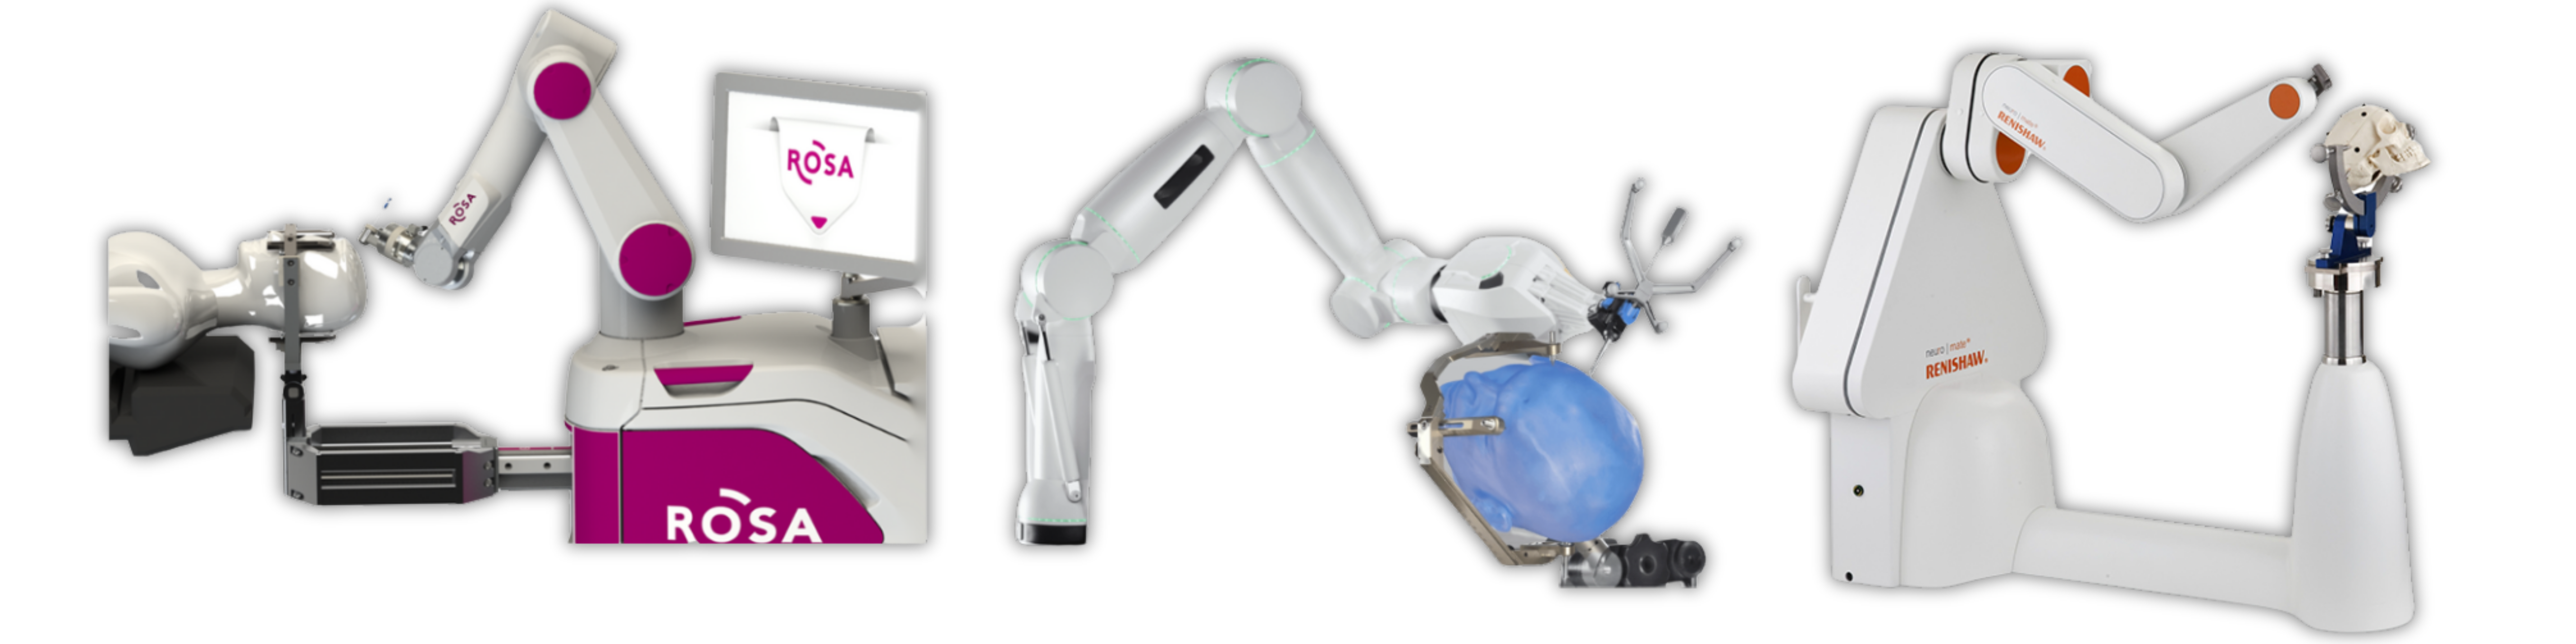
\includegraphics[width=0.99\textwidth]{USPSC-img/robots_enhanced.png}
     \caption{Competing robots capable of performing SEEG surgeries: Zimmer Biomet ROSA ONE Brain, Brainlab Cirq and Renishaw Neuromate respectively.}
     \label{fig:robots}
\end{figure}

The literature presents developments of \textit{frameless} systems for SEEG surgeries focused on facilitating surgical procedures, increasing the precision and safety of surgery \cite{gonzalez2016technique} \cite{cardinale2013stereoelectroencephalography}. The pioneering robot introduced to the market capable of performing SEEG neurosurgery was Renishaw's Neuromate in 1998 \cite{cardinale2013stereoelectroencephalography}. Figure \ref{fig:robots} presents the system, featuring a triangular base and a Mayfield or Leksell support for fixing the skull. Another system developed by Medtech in France and acquired by Zimmer Biomet was ROSA ONE Brain, also capable of performing SEEG surgeries. Later, Brainlab also developed Cirq for use in surgeries such as SEEG. It is worth mentioning that the three systems are compatible, in addition to SEEG, with brain biopsy surgeries and DBS (widely used in the treatment of Parkinson's).

% neuromate
Neuromate was the first neurosurgery robot to be commercially developed, but it also presents challenges in its application \cite{kajita2015installation}. The biggest challenge is the need for an exclusive operating room for the robot, due to the inability to move the system. This makes the hospital's logistics difficult and makes purchasing it impossible due to this restriction. Furthermore, one of the biggest difficulties with Neuromate is the need for a dedicated operating room for the robot, without the possibility of moving it between operating rooms. Moreover, Neuromate has only 5 degrees of freedom (DOF), constituting an under-actuated robotic system, losing mobility and positioning capacity in relation to conventional robotic systems (with 6 DOF).

% cirq
The Cirq robotic system is used as a neuronavigation tool. A device with reflective spheres is fixed to the robot's flange, similar to that used in common neuronavigators. This device is viewed by an infrared stereo camera and the position of the tool is calculated. Each joint of the robot has only brakes and, therefore, is not actuated, but allows the system to remain static during procedures.

Its adjustment is done semi-automatically, where the surgeon approaches the robot to the desired position and the robot adjusts itself with an actuator fixed to its flange. The neuronavigator is used to operate this system, which has: a camera carriage; a screen carriage; and a robotic manipulator fixed to the operating table. Combined with other devices present in the operating room, these three devices bring difficulties in logistics and in organizing the space in the room compared to systems that have only one carriage. Finally, the cost of the complete system is comparatively higher than that of competitors on the market.

ROSA ONE Brain, even though it doesn't have the disadvantages present in other systems, has its own problems. The system, unlike Cirq, for example, is not collaborative. In other words, even though it is designed to perform a task together with the surgeon, ROSA does not feature sensors that are present in collaborative systems, such as measuring joint torque, collision detection, and automatic braking when an emergency is activated. This aspect makes ROSA a conventional robot applied to collaborative tasks, putting doctor and patient safety at risk. Yara, the system proposed in this project, uses collaborative systems, validated worldwide for tasks that involve joint operations with humans, ensuring the surgeon's safety.

ROSA is not collaborative, constituting an industrial system that has limited capacity to understand the surrounding environment, putting patient and doctor safety at risk. Conventional, non-collaborative industrial robots must be isolated from humans at a safe distance in their workspace for most workplace safety regulations in the world. This concept has not been applied to surgical robots as they are not under industrial legislation. In the literature, the use of collaborative systems for neurosurgery within commercial systems was not identified. KUKA was a pioneer in the development of collaborative systems approved by international regulations for medical applications with the KUKA LBR Med. This increases safety in robotic manipulation during surgeries, unlike existing systems on the market.

The presence of robots for stereotactic surgeries in Brazil and developing countries is still timid at the moment. Figure \ref{fig:robots} presents competing robots and their incidence in hospitals in Brazil. According to our investigation, there are no hospitals that have purchased ROSA or Neuromate in the country. Cirq was acquired by Hospital Moinho de Vento in Rio Grande do Sul in 2022, in addition to having performed some surgeries in other hospitals in the country. This represents a marketing opportunity, as entry into the Brazilian brand is difficult without technical support from the manufacturers of ROSA and Neuromate in the country. With this, Yara aims to meet the demand for improving SEEG procedures in the country in the short term, in Latin American countries in the medium term and in other continents in the long term.

\subsection{Mechatronic Systems and Planning Software}

The Stealth AutoGuide - Medtronic \cite{medtronic} is not a robotic arm, but is defined as a robotic system coupled to the apparatus that fixes the patient's head (Mayfield, Leksell or CRW) and assists the surgeon in aligning the final trajectory of each electrode. Lastly, software that assists in planning the surgery by calculating the coordinates for the stereotactic apparatus also qualify as less sophisticated but more accessible competitors. Brainlab Elements is an example of a computer-assisted method that presents advanced functionalities and excellent usability. Renishaw's Neuroinspire is also a renowned cranial planning system. Mevis' MNPS is presented as a national solution for planning brain neurosurgeries. However, all of these software programs are dependent on the stereotactic apparatus and the difficulties pointed out in Section \ref{sec:stereotatics}.

\section{Introducing Yara}

Yara presents itself as a robotic platform that is able to perform frameless procedures, reducing risks, surgery time and increasing precision in relation to frame-based procedures. A collaborative system, which maintains the surgeon's safety, while allowing better usability and manipulation of the robotic system. The system has software that allows surgery planning with the entry and target points of each desired electrode, the fusion of MRI and CT images, automated registration using depth cameras and collision-free movement of the robot for alignment to the desired trajectory. Furthermore, Yara also works as a neuronavigator, increasing the number of surgeries supported. The surgeon can move the robot with his hands, as in the neuronavigation process, and use the brakes to lock the desired position. In this way, Yara presents itself as an innovation in the field of stereotactic surgeries, surpassing the limits of state-of-the-art robotic systems.

% %%%%%%%%%%%

The \textit{Yara} system, proposed in this project, should begin applications for SEEG and should extend its capacity to biopsy and DBS surgeries once validated in humans this year. This initial step is mainly due to SEEG surgery having slightly more lenient requirements in terms of accuracy than DBS and biopsy. Completing the SEEG validation stage, tests will be carried out for DBS and biopsies for validation and, with this, our system is on par with competitors such as ROSA, Neuromate and Cirq in terms of supported surgeries.